\begin{frame}[allowframebreaks]{\underline{Parameterization} -}
    \section{Parameterization}
    
\underline{Free Form Deformation technique :} FFD is a process by which shape to given geometry is achieved by manipulating the
location of control points. 
\begin{itemize}
\item It is easy to implement.
\item  More flexible while perturbating control points.
\end{itemize}
\vspace{1mm}
\underline{The 3D FFD equation:} 
  \begin{equation}
\mathbf{X}_{(u, t, s)}=\sum_{i=0}^{m} \sum_{j=0}^{n} \sum_{k=0}^{p} f_{i}^{m}(u) g_{j}^{n}(t) h_{k}^{p}(s) \mathbf{P}_{(i, j, k)}
\label{ffd_3d}
\end{equation}
where $\mathbf{P}_{(i, j, k)}$ is perturbed control points, $\mathbf{X}_{(u, t, s)}$ new coordinates of wing surface points, and Bernstein's polynomial $f_{i}^{m}(u)$ is defined as,
\begin{equation}
f_{i}^{m}(u)=\frac{(m) !}{(i) !(m-i) !} u^{i}(1-u)^{m-i}
\label{bernstein_poly}
\end{equation}

\begin{figure}
\parbox{0.49\linewidth}
{
\centering
 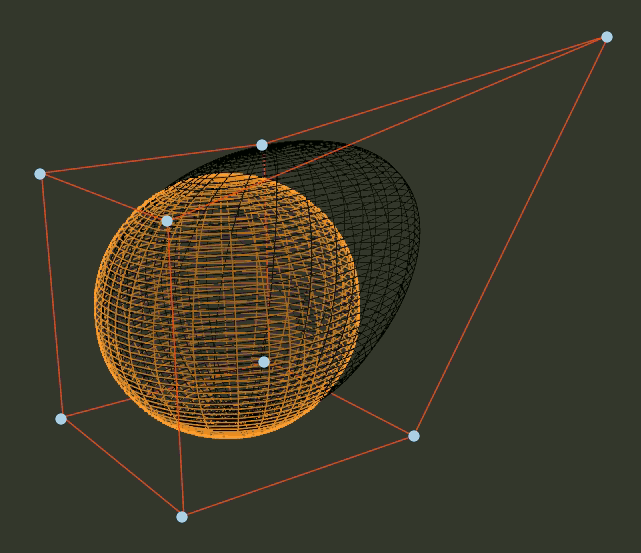
\includegraphics[scale = 0.15]{figures/sphere_ffd.png}
 \caption{Influence of the control point over the sphere body with $a^{(m,n,p)}$ as $2 \times 2 \times 2$ control points.}
 \label{sphere_ffd}
}
\parbox{0.47\linewidth}
{
\centering
   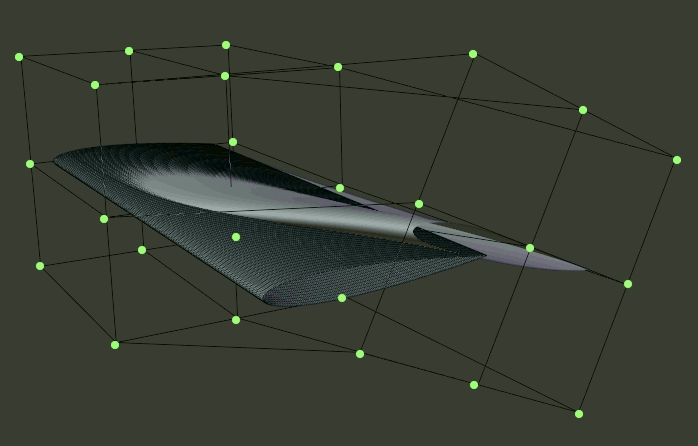
\includegraphics[scale = 0.15]{figures/ffd_wing.png}
  \caption{FFD of a wing shape, with the control points on the face of the wing-tip end are rotated and translated.}
  \label{wing_ffd}
}
\end{figure}
\begin{itemize}
    \item Figure \ref{sphere_ffd} represents the effect of control point perturbation over sphere.
    \item The effect of perturbation diminishes with distance from control point perturbed.
    \item Introducing more control points will provide better control over shape.
\end{itemize}

\begin{figure}
    \parbox{0.35\linewidth}
    {
    \centering
    \framebox{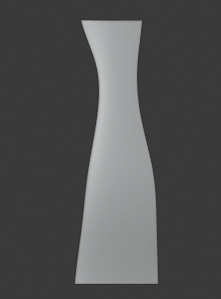
\includegraphics[scale=0.4]{figures/wing6_span.png}}
    \caption{Span view of wing 2.}
    \label{wing2_span}
    }
    \parbox{0.6\linewidth}
    {
    \centering
    \framebox{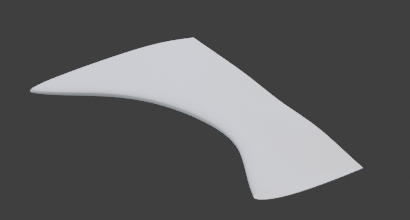
\includegraphics[scale = 0.4]{figures/wing2_iso.png}}
    \caption{Iso view of wing 1.}
    \label{wing1_iso}
    }
\end{figure}
\begin{itemize}
\item Figure \ref{wing2_span} and \ref{wing1_iso} illustrates the wings obtained with 60 control points.
\item With proper tuning of limits, it is possible to obtain twist, dihedral, taper characteristic to the wing.
\end{itemize}

\end{frame}